\chapter{Algoritmos}\label{chapter:algorithms}

\section{DP/DPLL}

\subsection{Principio de Resolución (PR)}
El Principio de Resolución (PR) fue una de las primeras técnicas aplicadas para intentar resolver SAT.

Dada una fórmula de la Lógica Proposicional escrita en Forma Normal Conjuntiva (FNC), esta se representa en su forma conjuntual, donde cada cláusula constituye un conjunto de literales y la fórmula en general es un conjunto de conjuntos. Gracias al concepto de ``conjunto'' esta representación evita la repetición de literales en las cláusulas, así como aquellas que aparezcan más de una vez en la FNC. 

Tomando esta representación como entrada, PR busca iterativamente pares de clásulas que contengan literales opuestos, para a partir de ellas generar una nueva clásula que constituya la unión de ambas, quitando eliminando el literal en cuestión y su opuesto. Es decir:

Sean $\textbf{B}$ y $\textbf{C}$ dos cláusulas de la FNC $\textbf{A}$, tales que $l \in \textbf{B}$ y $\neg l \in \textbf{C}$, donde $l$ es un literal y $\neg l$ su opuesto; entonces la cláusula resultante sería: $\textbf{D} = (\textbf{B}-{l}) \cup (\textbf{C}-{\neg l})$. Aquí las cláusulas $\textbf{B}$ y $\textbf{C}$ se denominan ``cláusulas padres'' o ``premisas'' y $\textbf{D}$ constituye el ``solvente'' o ``conclusión'' de $\textbf{B}$ y $\textbf{C}$.

Téngase en cuenta el siguiente ejemplo para una mejor comprensión.

$\dfrac{{\neg p, \neg q, \neg r},{\neg p, q, \neg r}}{{\neg p, \neg r}}$

$\dfrac{{\neg q}, {q}}{{}}$

El objetivo principal de PR es refutar $\textbf{A}$ si esta es insatisfacible, derivando una cláusula vacía (${}$). Es decir, si ${} \in \textbf{A}$ entonces $\textbf{A}$ es insatisfacible, y si ${} = \textbf{A}$ entonces $\textbf{A}$ es satisfacible.

\subsubsection{Resolución Unitaria (RU)}
Un caso particular de PR es Resolución Unitaria (RU), donde una de las ``cláusulas padres'' es una cláusula unitaria \footnote{Cláusula que contiene un único literal, por ende su valor se ve forzado a ser 1.} Por ejemplo:

$\dfrac{{\neg q, p, \neg r},{r}}{{\neg q, p}}$

\subsection{Davis-Putnam (DP)}
Uno de los primeros algoritmos para resolver SAT fue Davis-Putnam (DP), donde PR constituye uno de sus pilares. DP realiza tres procedimientos fundamentales: Propagación Unitaria (PU), Eliminación de Literales Puros (ELP) y Resolución Basada en División (RD). PU busca en la FNC de entrada clásulas unitarias y procede a eliminarlas de la fórmula, además de eliminar el literal complemntario de cada cláusula donde aparezca. ELP busca los literales que tengan una única polaridad en toda la fórmula (no exista su complementario) y procede a eliminar aquellas cláusula que contengan literales puros. Ambas, PU y ELP, son preprocesamientos que buscan simplificar lo más posible la FNC. Una vez realizados, DP procede con RD donde asigna un valor (0 o 1) a una variable y continúa recursivamente aplicando DP hasta encontrar poder decidir si la FNC es satisfacible o no. Véase el ejemplo a continuación:

Sean las siguientes, fórmulas de la Lógica Proposicional

$r, [q \land r] \implies p, [q \lor r] \implies \neg p, [\neg q \land r] \implies \neg p, \neg s \implies p$

A paritr de la conjunción de estas, se obtiene la siguiente FNC:

${\{r\}, \{p,\neg q, \neg r\}, \{\neg p, \neg q\}, \{\neg p, \neg r\}, \{\neg p,q,\neg r\}, \{p,s\}}$


Aplicando \textbf{PU} en ${r}$:

${{p,\neg q},{\neg p,\neg q},{\neg p},{\neg p,q},{p,s}}$

Aplicando \textbf{PU} en ${\neg p}$:

${{\neg q},{s}}$

Aplicando \textbf{PU} en ${\neg q}$:

${{s}}$

Aplicando \textbf{PU} en ${s}$:

${}$

Luego la fórmula es satisfacible.


DP requiere una memoria exponencial ya que evalúa todas las posibles asignaciones para las variables, generando un árbol de decisión como espacio de búsqueda que crece exponencialmente.

\begin{figure}[ht]
    \centering
    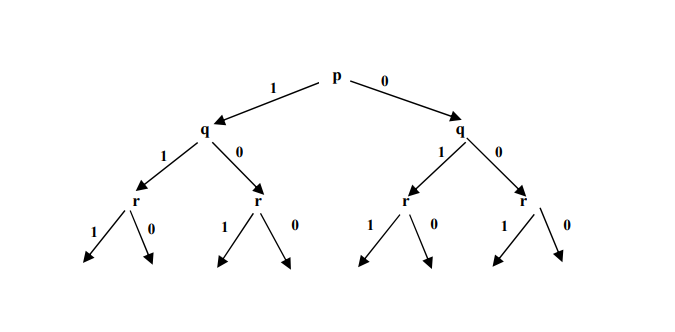
\includegraphics[width=0.8\textwidth]{Graphics/arboldp.png}
    \caption{Posible espacio de búsqueda de una FNC}
    \label{fig:arbol DP}
\end{figure}

\subsection{Davis-Putnam-Logemann-Loveland (DPLL)}
El algoritmo Davis-Putnam-Logemann-Lovelans (DPLL) aplica las mismas bases que DP, excepto que resuelve el problema de la memoria exponencial al realizar un \textit{backtrack} cronológico (al nivel anterior de decisión) en el árbol de asignaciones una vez encontrada una ``cláusula de conflicto''\footnote{Se denomina cláusula de conflicto a aquella cláusula cuyos literales evaluaron a 0 tras una asignación.}. Con este método, DPLL utiliza una estrategia \textit{``lazy''} para generar el árbol, dado que antes de ramificarse (otorgar un valor a una variable) verifica que no haya conflictos, garantizando que las asiganaciones válidas para la fórmula de entrada se encuentren en las hojas del árbol de decisión. Obsérvese que si un conflicto se produce en el nivel de decisión 0 y ambos valores para la variable ya han sido examinados, entonces se concluye que la fórmula es insatisfacible. Este proceso realizado por DPLL se denomina ramificación + propagación unitaria + retroceso.

Cabe destacar que DPLL tiene una etapa de preprocesamiento de la FNC, sobre la cual se aplican leyes de la Lógica Proposicional, así como se eliminan cláusulas redundantes mediante la aplicación de la subsunción de cláusulas\footnote{Sean $C$ y $C'$, cláusulas de una FNC; si $C' \subseteq C$, entonces se elimina $C'$ de la FNC.}. 

Obsérvese el siguiente ejemplo:

Sea la FNC:
${{\neg p,\neg q},{\neg p, \neg q},{\neg p,q,\neg r},{\neg p,r,s},{p,s}}$

Simplificando mediante la Ley de Absorción:

${{\neg p,\neg q},{\neg p,q,\neg r},{\neg p,r,s},{p,s}}$

Eliminando el literal puro $s$:

${{\neg p,\neg q},{\neg p,q,\neg r}}$

Ramificando: $p=1$

${{\neg q},{q,\neg r}}$

Aplicando PU:

${{\neg q},{q,\neg r}}$

Aplicando PU:

${\neg r}$

$\emptyset$

Luego la FNC es satisfacible.

No obstante la reducción del espacio de memoria de DPLL respecto a DP, aún quedan problemas fundamentales: selección de variables, \textit{backtrack} cronológico y selección de cláusulas unitarias.

En primer lugar la selección de la variable a asignar un valor influye en la ``forma'' que tomará el espacio de búsqueda, por lo que malas decisiones en este sentido conllevan a caminos más largos en la búsqueda de una solución. Análogamente se gana en eficiencia considerando heurísticas en la selección de variables. (poner ejemplo)

En segundo lugar, el \textit{backtrack} cronológico a partir de un conflicto obliga a explorar el resto de las posibles asignaciones de las variables en niveles anterirores, potencialmente, de forma innecesaria, sobre todo para aquellos casos donde la asignación causante del conflicto se encuentre a $k$ niveles de distancia del nivel del conflicto. Además, DPLL no aprovecha las cláusulas que han resultado conflictos, es decir, no aprende de ellas, por lo que es vulnerable a cometer el mismo error (mismo patrón incorrecto de asignaciones para las variables involucradas en el conflicto). Esto lo hace susceptible a repetir errores de forma recurrente.

Finalmente, el problema de selección de cláusulas unitarias, influye también en la eficiencia del algoritmo. Se puede decir que guarda relacón con la estrategia de selección de variables.

\section{CDCL}
CDCL es una mejora que se le añadió al algoritmo DPLL con el objetivo de erradicar el problema del retroceso (\textit{backtrack}) cronológico, una vez encontrada una cláusula de conflicto (todos sus literales evalúan 0).

El retroceso cronológico consiste en recorrer el árbol de decisión (estructura propia del algoritmo DPLL que se forma al asignarle valores a las variables) retrocediendo de a 1 por cada nivel, probando todos los valores de cada variable hasta encontrar la asignación causante del conflicto. Esta búsqueda es ineficiente dado que, además de analizar casos innecesarios, vuelve a cometer el mismo error (potencialmente realiza la misma combinación de asignaciones) generando búsquedas redundantes.
Para solucionar este problema, CDCL crea un grafo dirigido y acíclico que permite guardar el historial de asignaciones de cada variable. En dicho grafo, los nodos son las variables y los arcos constituyen la causa de la asignación de dicha variable: la cláusula a la que pertenece, si fue asignada por propagación unitaria, y null para variables asignadas por decisión. El grafo también contiene 2 metadatos: el valor asignado a cada variable (0 o 1), y el nivel de decisión en el que se asignó (los diferentes niveles de decisión están marcados por la asignación de valores por decisión). Cabe destacar que la dirección de los arcos en el grafo va desde las variables de decisión hacia aquellas que, en el mismo nivel, tuvieron que forzar su valor por propagación unitaria. En el caso de una nueva variable de decisión, se crea un nuevo arco con valor nulo desde la variable asignada por decisión en el nivel anterior, hasta la nueva variable.

Cuando una cláusula resulta ser de conflicto (sus literales evaluaron 0), CDCL crea un nuevo nodo en el grafo que representa dicho conflicto, para comenzar con su análisis.
Este análisis busca en el grafo la asignación causante del conflicto, para retroceder justo hacia ese punto y realizar un \textit{backjump} en lugar de un retroceso cronológico, como en DPLL. Asimismo, con este análisis CDCL busca conformar una cláusula (cláusula aprendida) que represente la combinación de asignación de valores que condujo a dicho conflicto, para incluirla en la base de datos de las cláusulas de la FNC y evitar cometer el mismo error en iteraciones futuras. El punto escogido para realizar el \textit{backjump} es conocido como primer punto de implicación único (\textit{First-UIP} por sus siglas en inglés). Este punto, será aquel literal que en la cláusula aprendida, posea el más alto nivel de decisión, diferente del actual.

Es necesario enfatizar en el hecho de que la cláusula aprendida debe contener únicamente 1 literal cuyo valor haya sido asignado en el nivel de decisión actual. En caso de haber más de uno, CDCL recorre el grafo en busca de la cláusula que causó la asignación de una de estas variables y aplica el Principio de Resolución entre esta y la cláusula aprendida hasta el momento. La cláusula resultante pasará a ser la nueva cláusula aprendida. El proceso se repetirá hasta que la cláusula aprendida contenga solo un literal cuyo valor fue asignado en el nivel de decisión actual.

En caso de que el nivel del \textit{backjump} sea el nivel 0, CDCL considera la FNC como insatisfacible.

(poner ejemplos)


\section{DLIS}

\section{VSIDS}

\section{Reinicio (\textit{restarts})}

\section{Selección de cláusulas unitarias}